\chapter{碳钢退火、正火后的组织观察与硬度分析}
\section{实验目的}
    \begin{enumerate}
        \item 了解碳钢的退火、正火过程。
        \item 观察和研究碳钢经不同退火处理、正火处理后显微组织的特点,分析热处理工艺对其组织与硬度的影响,并了解退火、正火的应用领域。
    \end{enumerate}
\section{实验原理}%简单描述,含必要的公式和附图;
    热处理是一种很重要的热加工工艺方法。热处理的主要目的是改变钢的性能,其中包括使用性能及工艺性能。绝大多数重要的机械零件在制备过程中都要经过热处理,其目的就是把工件加热到一定温度,然后根据不同的要求采取不同的保温时间、冷却速度,使金属零件中的结构产生预期的变化,从而使零件具有不同的机械性能。\par
    热处理包括四个因素:加热速度、最高温度、加热时间(通常将工件升温和保温所需时间算在一起,统称为加热时间)和冷却速度。根据热处理工艺的使用和进行方式不同,热处理一般可分为下列四种类型:退火、正火、淬火、回火。\par
    \subsection{退火}
        退火是将工件加热到适当温度,根据材料和工件尺寸采用不同的保温时间,然后进行缓慢冷却(冷却速度最慢),目的是使工件内部组织达到或接近平衡状态,获得良好的工艺性能和使用性能,或者为进一步淬火过程作组织准备。退火的工艺方法有很多种,其中包括完全退火、不完全退火、球化退火和去应力退火等。在实际生产中,经常采用退火作为预备热处理工序,安排在锻造、铸造等热加工之后,切削加工之前,为下一道工序作组织和性能上的准备。
        \subsubsection{完全退火}
            将亚共析钢件加热到 $A_3+(30\sim 50)~\unit{\degreeCelsius}$($A_3$ 线是钢 $\alpha$ 固溶体转变为 $\gamma$ 固溶体之临界温度),保温一段时间,然后缓慢地随炉冷却的工艺方法。
        \subsubsection{不完全退火}
            将亚共析钢加热到 $A_1 \sim A_3~\unit{\degreeCelsius}$($A_1$ 为共析转变温度),过共析钢加热到 $A_1 \sim A_{\textrm{cm}}~\unit{\degreeCelsius}$(碳在奥氏体中的溶解度曲线所对应的温度为 $A_{\textrm{cm}}$ 温度),保温后缓慢冷却的方法。
        \subsubsection{球化退火}
            将过共析钢件加热到 $A_1+20~\unit{\degreeCelsius}$ 左右,保温一定时间后以适当的方式冷却使钢中的碳化物球状化的工艺方法。
        \subsubsection{去应力退火}
            将钢件加热到相变点 $A_1$ 以下的某一温度,保温一定时间后缓慢冷却的工艺方法。其目的是为了消除由于冷热加工所产生的残余应力。一般碳钢和低合金钢加热温度为 $550 \sim 600~\unit{\degreeCelsius}$,而高合金钢一般为 $600 \sim 700~\unit{\degreeCelsius}$,保温一定时间(一般近 \SI{3}{\minute/\milli\metre}),然后随炉缓慢冷却($\le \SI{100}{\degreeCelsius/\hour}$)到\SI{200}{\degreeCelsius}出炉。对于铸铁件一般加热到 $500 \sim 550~\unit{\degreeCelsius}$,不能超过 \SI{550}{\degreeCelsius},因为超过 \SI{550}{\degreeCelsius} 以后铸铁中的珠光体要发生石墨化。
        \subsubsection{扩散退火}
            又称均匀化退火,用于合金钢锭和铸件,以消除枝晶偏析,使成分均匀化。扩散退火是把铸锭或铸件加热到略低于固相线以下某一温度,通常为 $A_3$ 或 $A_{\textrm{cm}} + (150 \sim 300)~\unit{\degreeCelsius}$,长时间保温后随炉缓慢冷却的一种热处理工艺方法。一般碳钢采用 $1100 \sim 1200~\unit{\degreeCelsius}$,合金钢采用 $1200 \sim 1300~\unit{\degreeCelsius}$,保温时间为 $10 \sim 15~\unit{\hour}$。
    \subsection{正火}
        正火是退火的特殊形式,其与一般退火所不同之处是试样在具有稍大的冷却速度的空气中进行冷却。\par
        正火加热温度选择:正火则是将钢材加热到 $A_3$ 或 $A_{\textrm{cm}} + (30 \sim 50)~\unit{\degreeCelsius}$,保持一定时间后在空气中进行冷却。一般亚共析钢加热至$A_3 + (30 \sim 50)~\unit{\degreeCelsius}$;过共析钢加热至 $A_{\textrm{cm}} + (30 \sim 50)~\unit{\degreeCelsius}$,即加热到奥氏体单相区。退火和正火加热温度范围选择见\fgref{fig:1}。
        \begin{figure}[!ht]
        \begin{floatrow}\centering
            \ffigbox[60mm]{\caption{退火和正火的加热温度范围\label{fig:1}}}{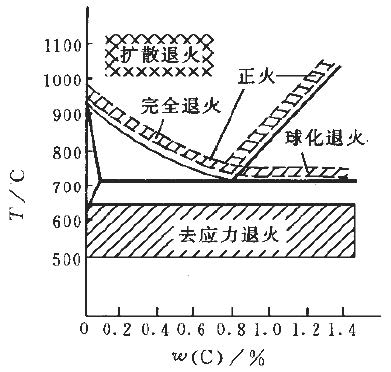
\includegraphics[height=40mm]{img/A3/fig1.jpg}}
            \ffigbox[\Xhsize]{\caption{碳钢热处理后的金相组织($450\times$)。(a) T12 钢球化退火,(b) 45 钢正火\label{fig:2}}}{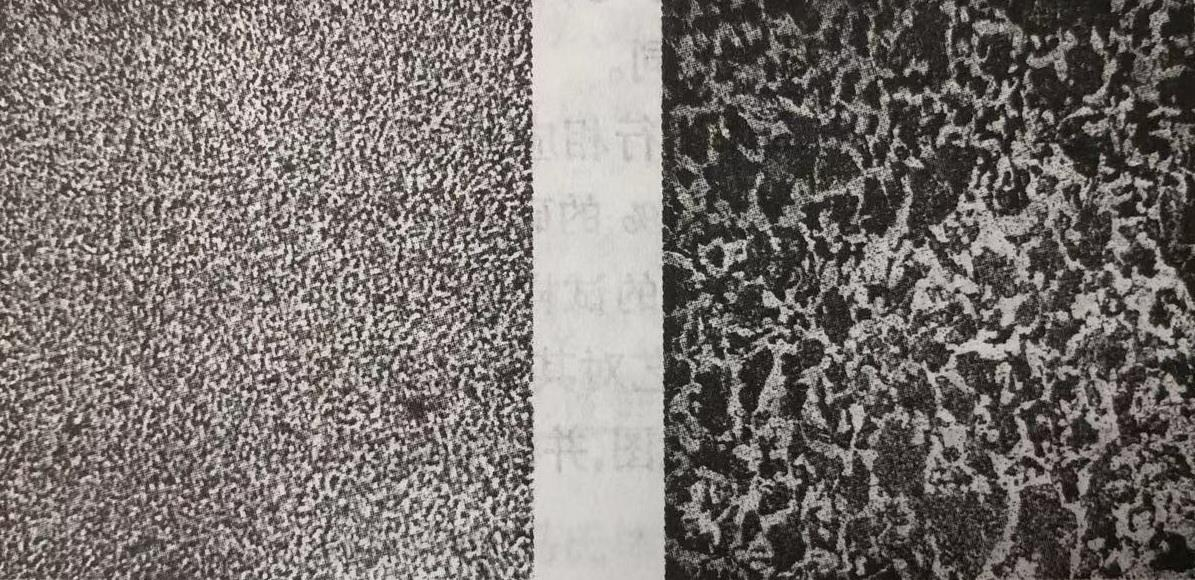
\includegraphics[height=40mm]{img/A3/fig2.jpg}}
        \end{floatrow}
        \end{figure}
    \subsection{退火与正火保温时间的确定}
        在装炉量不太大时,可用下式计算保温时间
        \begin{equation}
            \tau = K D \label{equ:A3.1}
        \end{equation}
        式中,$K$ 为加热系数,一般 $K=1.5 \sim \SI{2.0}{\minute/\milli\metre}$;$D$ 为工件有效尺寸。合金钢的保温时间比碳钢长一些,工件越大,装炉量越多,保温时间也越长。
    \subsection{碳钢退火、正火后的显微组织}
        亚共析碳钢一般采用完全退火,经退火后可得接近于平衡状态的组织,即铁素体加珠光体。过共析碳素工具钢则多采用球化退火,获得在铁素体基体上均匀分布着的粒状渗碳体的组织,称为球状珠光体或球化体。如 T12 钢经球化退火后组织为球状珠光体。二次渗碳体和珠光体中的渗碳体都呈球状(或粒状),如\fgref{fig:2}(a)所示,在铁素体基体上分布的颗粒状 \ce{Fe3C},铁素体基体上白色小颗粒为 \ce{Fe3C}。\par
        碳钢正火后的组织比退火的细,并且亚共析钢的组织中细珠光体(索氏体)的质量分数比退火组织中的多,并随着碳质量分数的增加而增加。45 钢正火组织为铁素体 $+$ 索氏体,如\fgref{fig:2}(b)。其中白色条状为铁素体,沿晶界析出;黑色块状为索氏体。正火冷速快,铁素体得不到充分析出,质量分数少,进行共析反应的奥氏体增多,析出的珠光体多而细。
    \subsection{注意事项}
    \begin{enumerate}
        \item 本实验加热为高温马弗炉,在放、取试样时一定要注意安全。
        \item 往炉中放、取试样必须使用夹钳,夹钳必须擦干,不得沾有油和水。
        \item 热处理后的试样均要用砂纸打磨掉表面黑色氧化皮后再测定硬度值
    \end{enumerate}
\section{实验仪器}%规格及参数
    箱式电阻加热炉,洛氏硬度计,砂纸,抛光机,金相显微镜。热处理试样:45 钢及 T12 钢。
\section{实验过程}%简述主要过程和实验内容
    \begin{enumerate}
        \item 每4人一组,领取45钢(2个)、T8(1个)及T12钢(1个)试样一套,每组共同完成一套实验(对应下表中相应的热处理工艺方法)。
        \begin{table}[!ht]\centering
            \caption{试样的热处理工艺}
            \begin{tabular}{|c|c|c|c|c|}\hline
                试样号码 & 钢号 & 热处理工艺 & 浸蚀剂 & 建议放大倍数 \\ \hline
                \Sam & 45 & 完全退火 & 4\% 硝酸酒精 & 200 $\sim$ 500 \\ \hline
                \Sam & 45 & 正火 & 4\% 硝酸酒精 & 200 $\sim$ 500 \\ \hline
                \Sam & T8 & 正火 & 4\% 硝酸酒精 & 200 $\sim$ 500 \\ \hline
                \Sam & T12 & 球化退火 & 4\% 硝酸酒精 & 200 $\sim$ 500 \\ \hline
            \end{tabular}
            \setcounter{sample}{0}
        \end{table}
        \item 制定热处理工艺参数,可参考以下工艺参数。
        \begin{enumerate}
            \item 45 钢完全退火工艺:加热温度为 $860 \pm \SI{10}{\degreeCelsius}$,根据试样有效尺寸计算保温时间,保温后炉冷到\SI{500}{\degreeCelsius}左右出炉空冷。
            \item 45 钢正火工艺:加热温度为 $860 \pm \SI{10}{\degreeCelsius}$,根据试样有效尺寸计算保温时间,保温后出炉空冷。
            \item T8 钢正火工艺:加热温度为 $820 \pm \SI{10}{\degreeCelsius}$,根据试样有效尺寸计算保温时间,保温后出炉空冷。
            \item T12 钢球化退火工艺:加热温度为 $760 \pm \SI{10}{\degreeCelsius}$,根据试样有效尺寸计算保温时间(约 40 分钟),保温后随炉冷却到 \SI{680}{\degreeCelsius} 保温 40 分钟,随后炉冷到 \SI{500}{\degreeCelsius} 出炉空冷。
        \end{enumerate}
        \item 利用硬度计对所有热处理后的试样进行硬度测试,每个试样至少三个试验点,再取一个平均值,分析热处理工艺对其硬度的影响。(硬度测试须在金相磨制观察前完成)
        \item 根据拟定的热处理工艺对试样进行相应的热处理工艺处理,然后利用金相砂纸对热处理后的\textbf{试样进行磨制、抛光},并用 4\% 的硝酸酒精进行腐蚀制得金相试样。利用金相显微镜对其进行\textbf{显微组织观察},分析热处理工艺对其组织的影响。
        \item 实验结束后,汇总各小组实验数据,根据实验数据分析冷却方法对碳钢性能(硬度)的影响,并阐明硬度变化的原因。
    \end{enumerate}
\section{实验数据}
\begin{table}[!ht]\centering
    \caption{不同热处理试样的硬度值}
    \begin{tabular}{|*{5}{c|}}\hline
        材料及热处理状态 & \multicolumn{3}{c|}{测得硬度数据} & 平均值 \bigstrut \\ \hline
        45 钢经完全退火 & 86.6 HRB & 84.0 HRB & 84.5 HRB & 85.0 HRB \bigstrut \\ \hline
        45 钢经正火 & 94.6 HRB & 94.8 HRB & 95.4 HRB & 94.9 HRB \bigstrut \\ \hline
        T8 钢经正火 & 33.5 HRC & 35.2 HRC & 33.5 HRC & 34.1 HRB \bigstrut \\ \hline
        T12 钢经球化退火 & 94.0 HRB & 94.1 HRB & 93.6 HRB & 93.9 HRB \bigstrut \\ \hline
    \end{tabular}
\end{table}
\begin{figure}[!ht]
    \caption{洛氏硬度计参数}
    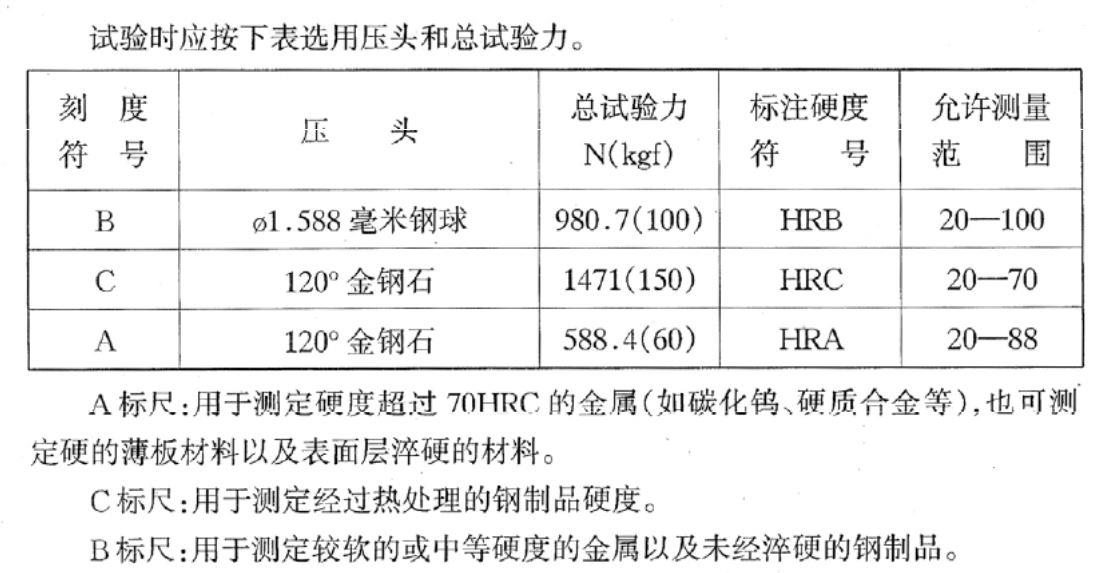
\includegraphics[width=\textwidth]{img/A3/fig3.jpg}
\end{figure}\clearpage
\section{样品显微组织}
\begin{figure}[!ht]
    \subfloat[45 钢完全退火 200x]{\includegraphics[width=0.35\textwidth]{img/A3/45tuihuo_200x.jpg}\label{expfig:45th200x}} \hspace{30pt}
    \subfloat[45 钢完全退火 500x]{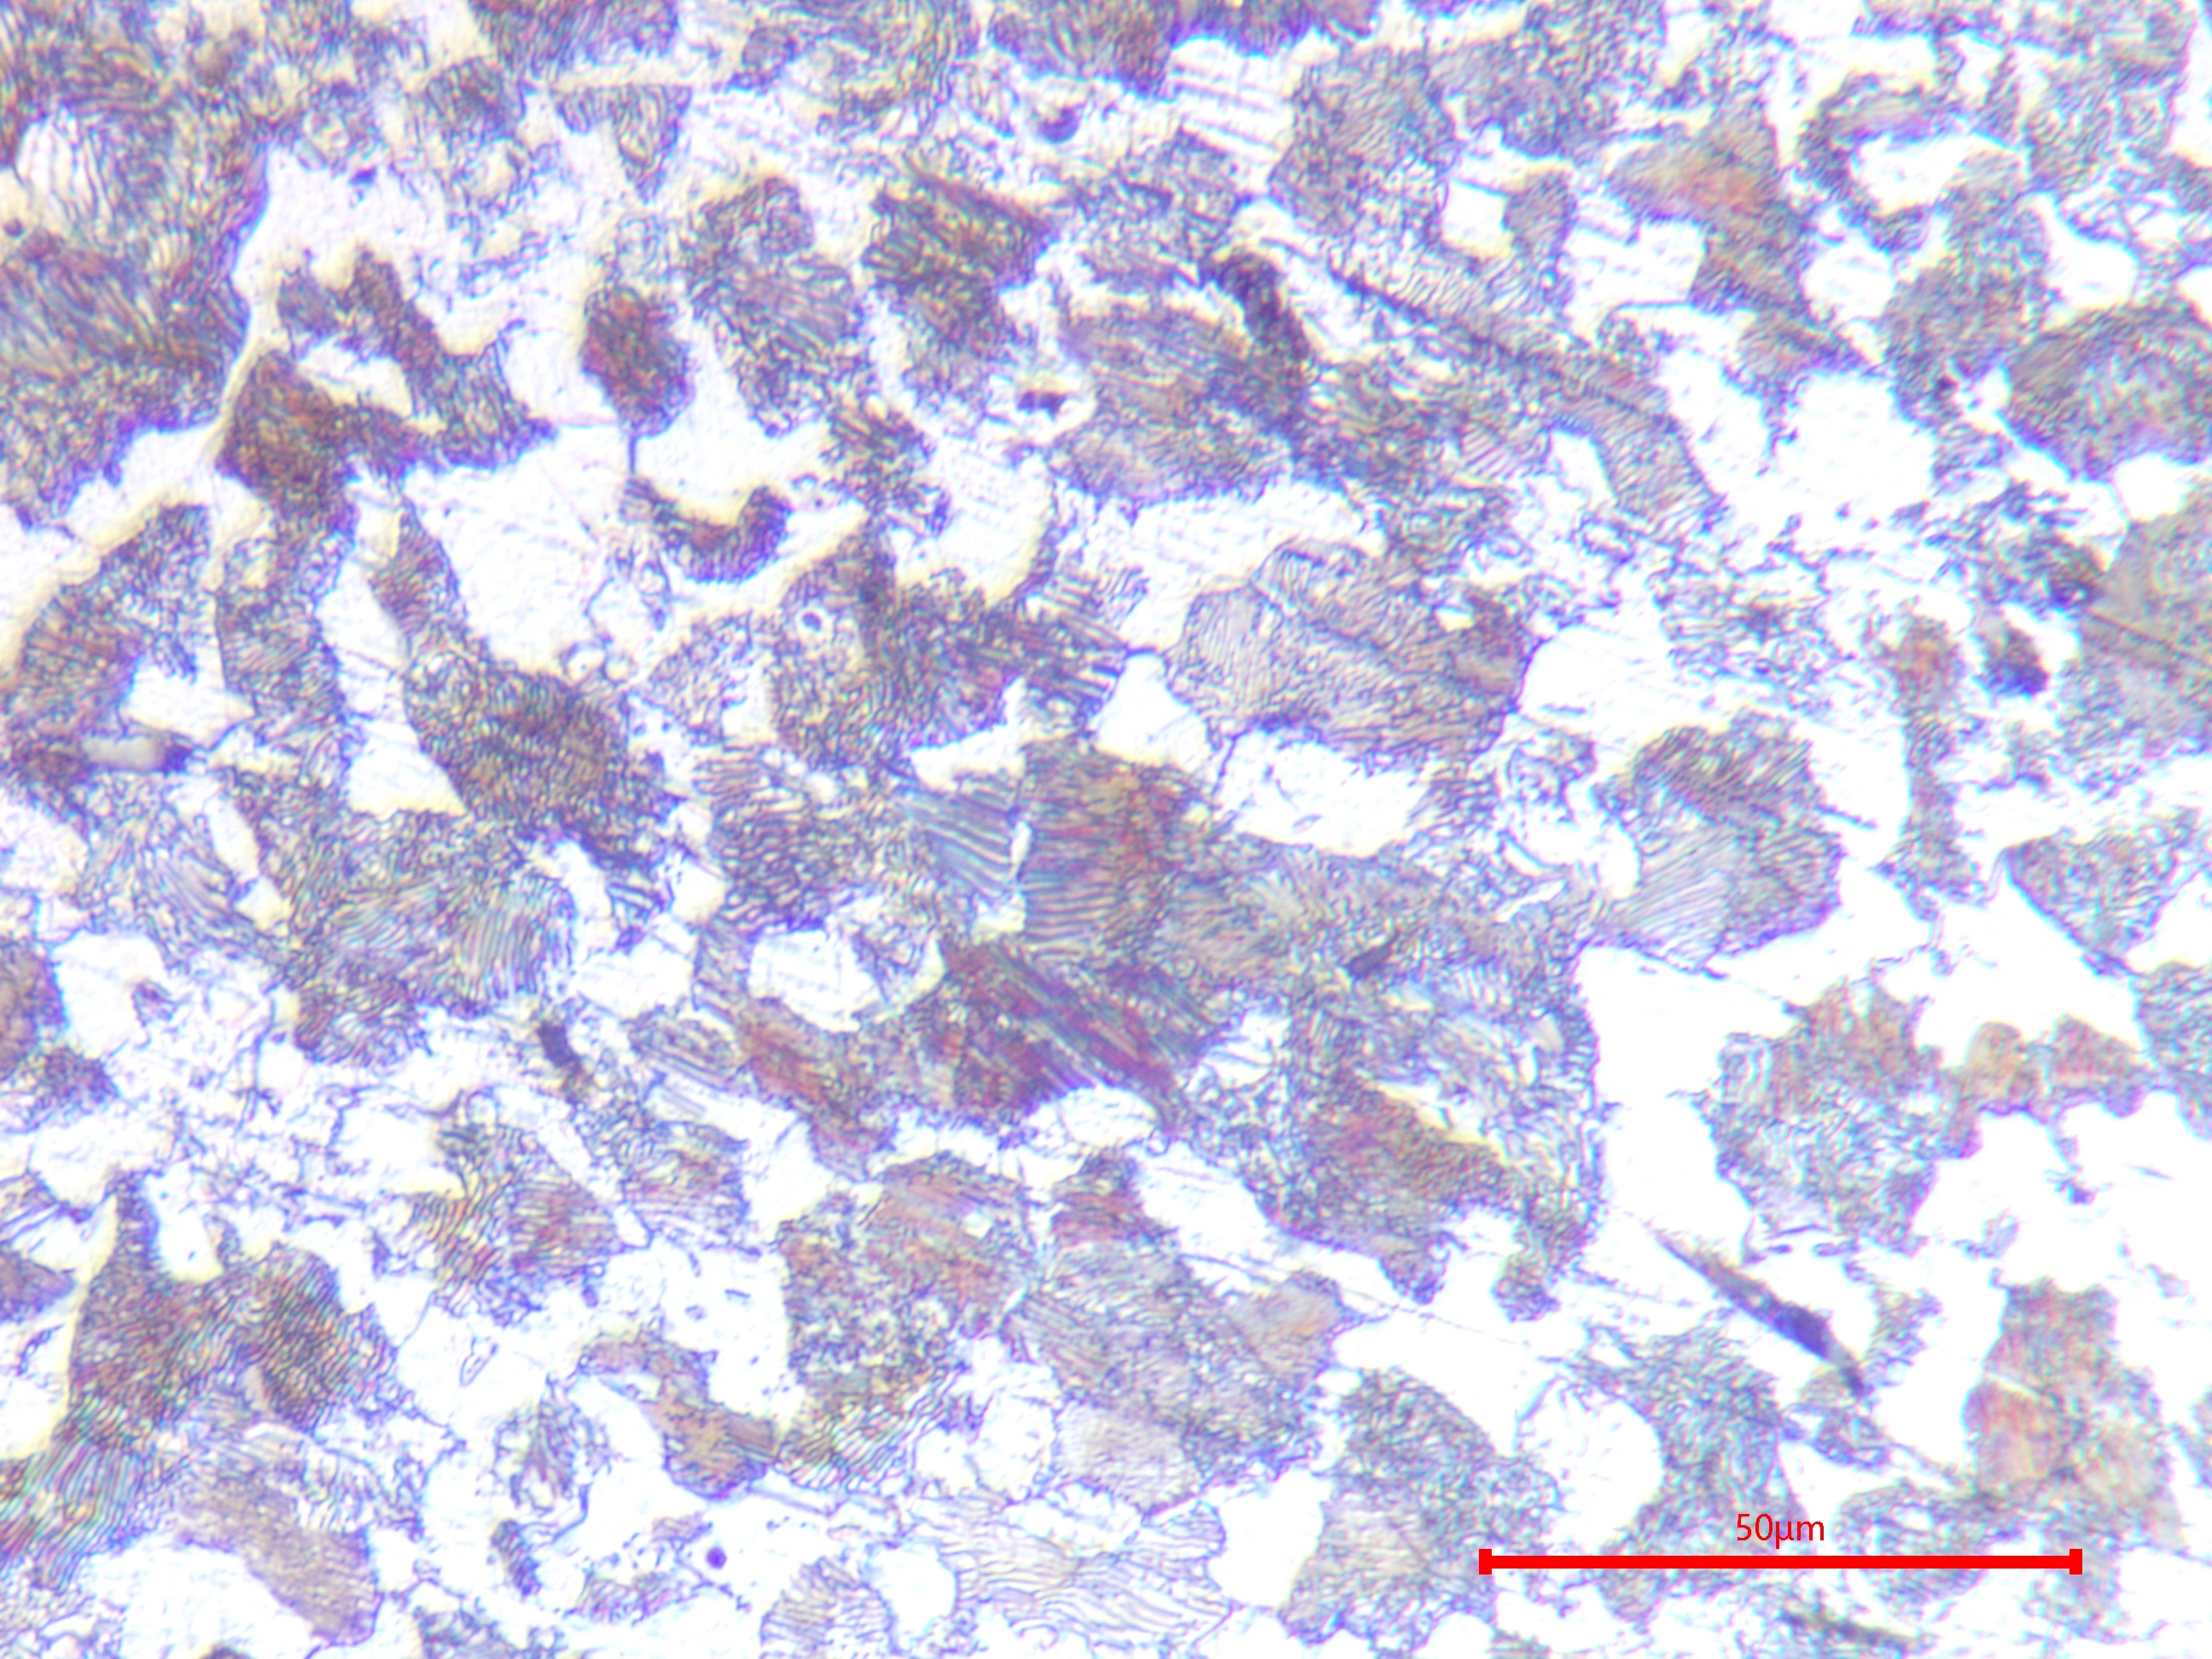
\includegraphics[width=0.35\textwidth]{img/A3/45tuihuo_500x.jpg}\label{expfig:45th500x}} \\
    \subfloat[45 钢正火 200x]{\includegraphics[width=0.35\textwidth]{img/A3/45zhenghuo_200x.jpg}\label{expfig:45zh200x}} \hspace{30pt}
    \subfloat[45 钢正火 500x]{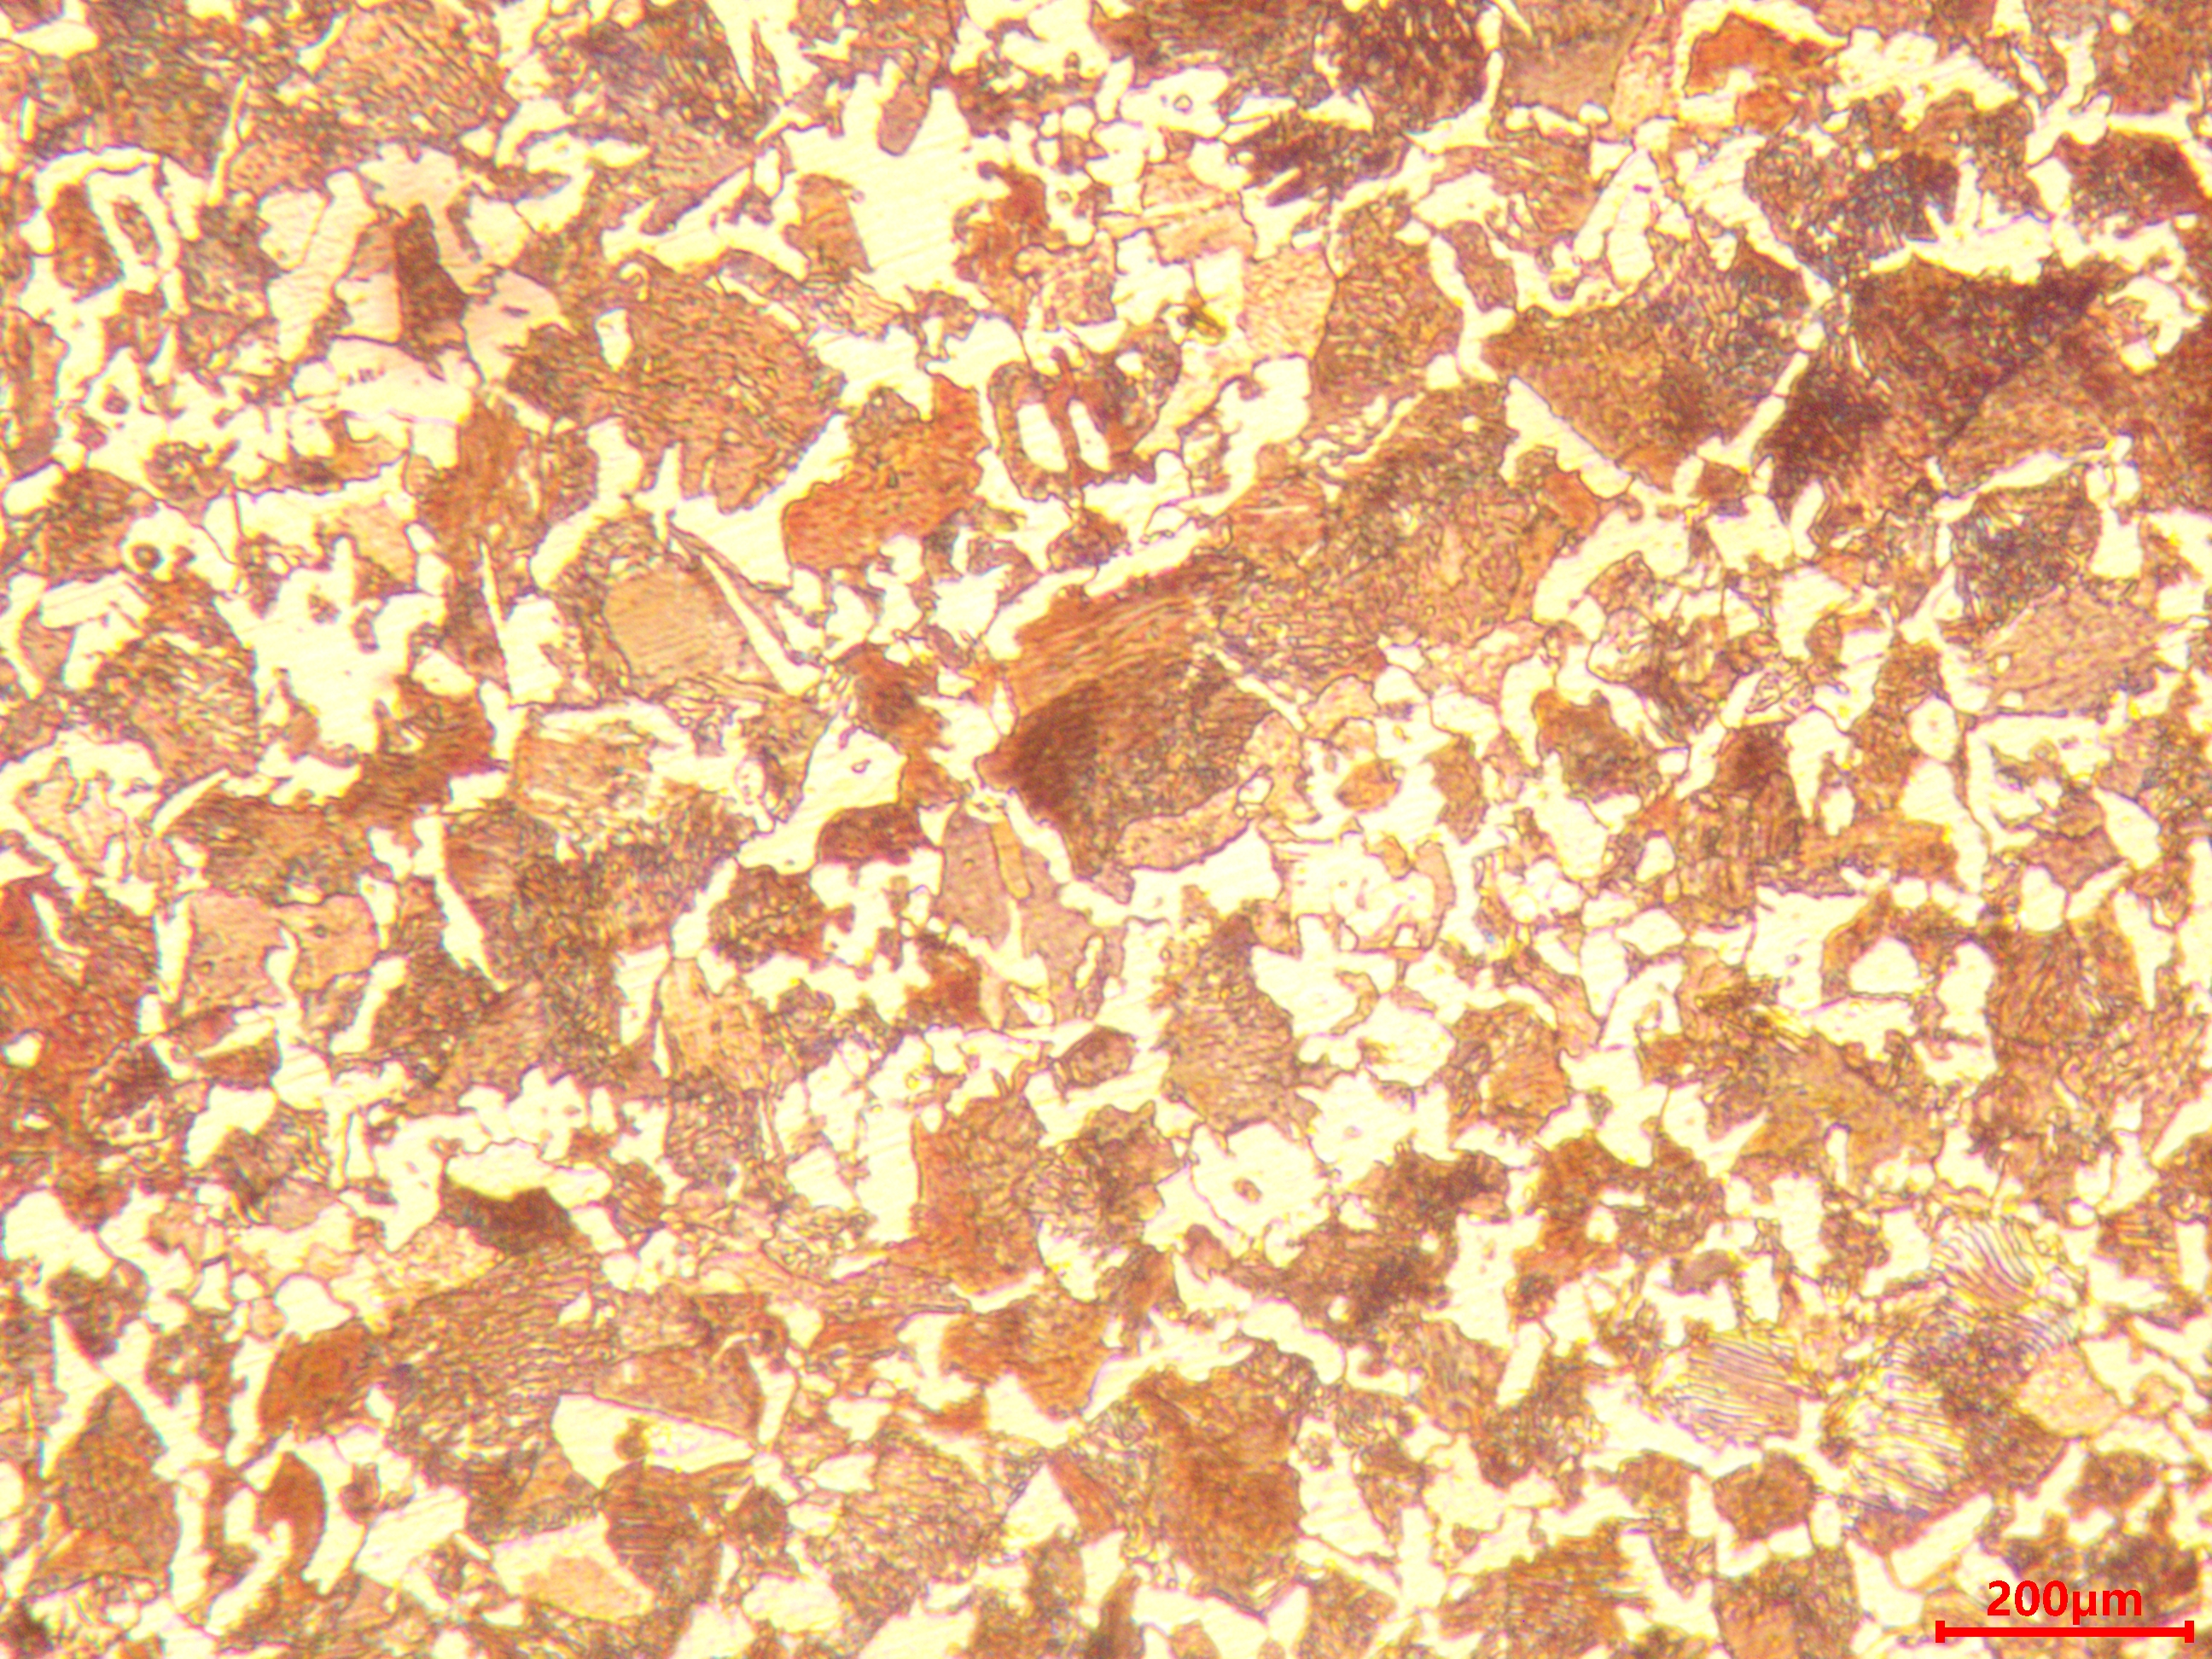
\includegraphics[width=0.35\textwidth]{img/A3/45zhenghuo_500x.jpg}\label{expfig:45zh500x}} \\
    \subfloat[T8 钢正火 200x]{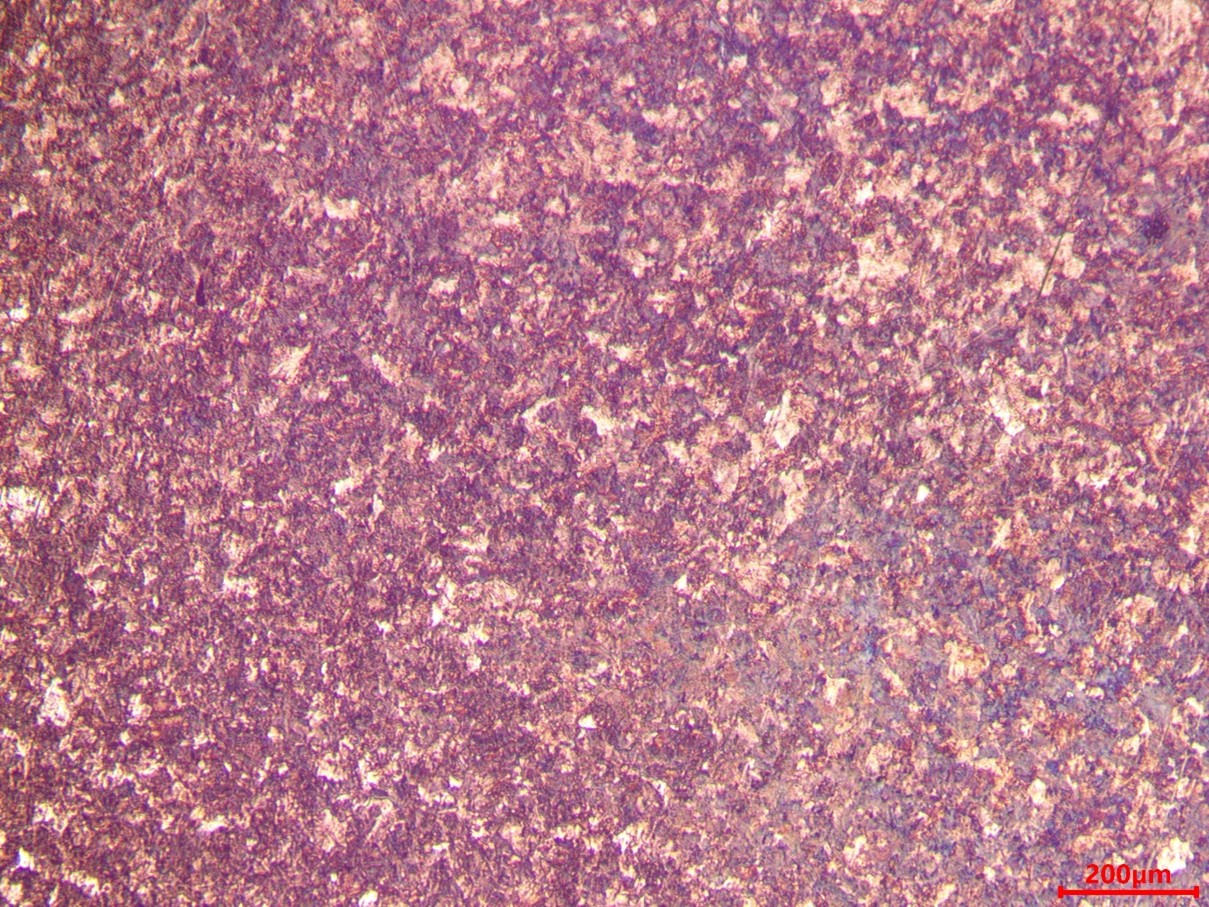
\includegraphics[width=0.35\textwidth]{img/A3/T8zhenghuo_200x.jpg}\label{expfig:t8zh200x}} \\
    \subfloat[T12 钢球化退火 200x]{\includegraphics[width=0.35\textwidth]{img/A3/qiu_T12_20x10x.jpg}\label{expfig:t12qh200x}} \hspace{30pt}
    \subfloat[T12 钢球化退火 500x]{\includegraphics[width=0.35\textwidth]{img/A3/qiu_T12_50x10x.jpg}\label{expfig:t12qh500x}} \\
\end{figure}
\section{组织分析}
45 钢在 $\SI{860}{\degreeCelsius}$ 完全退火的组织由白色不规则多边形铁素体和深色片层状珠光体组成,硬度在 85 HRB 左右,如\fgref{expfig:45th200x} 和\fgref{expfig:45th500x} 所示。\par
45 钢在 $\SI{860}{\degreeCelsius}$ 正火的组织由白色块状和网状铁素体及深色细片状珠光体组成,硬度在 95 HRB 左右,如\fgref{expfig:45zh200x} 和\fgref{expfig:45zh500x} 所示。\par
T8 钢在 $\SI{820}{\degreeCelsius}$ 正火的组织由珠光体和层状渗碳体组成,硬度在 34 HRB 左右,如\fgref{expfig:t8zh200x} 所示。\par
T12 钢在 $\SI{760}{\degreeCelsius}$ 完全退火的组织由等轴状晶粒的铁素体和细小颗粒状分布的渗碳体组成,硬度在 94 HRB 左右,如\fgref{expfig:t12qh200x} 和\fgref{expfig:t12qh500x} 所示。\par
\section{实验思考与讨论}
\begin{enumerate}
    \item \thinking{45 钢常用的热处理是什么?它们的组织是什么?有何工程应用?}{45 钢常用的热处理包括正火和淬火。正火是将钢加热至临界温度后冷却,以调节其组织和硬度。淬火是将钢迅速冷却,使其组织转变为马氏体结构,从而提高钢的硬度和强度。45 钢经过正火处理后组织为白色块状和网状铁素体及深色细片状珠光体。它常用于制造轴承、齿轮、螺栓、销子、传动轴等要求高强度和耐磨性的零部件。}
    \item \thinking{退火状态的 45 钢试样分别加热到 $\SI{600}{\degreeCelsius} \sim \SI{900}{\degreeCelsius}$ 之间不同的温度后,在水中冷却,其硬度随加热温度如何变化?为什么?}{随温度的升高而提升。\SI{600}{\degreeCelsius} 左右为珠光体,升高温度变为未溶铁素体和马氏体,再升高为马氏体。}
    \item \thinking{T12钢经球化退火后得到的组织在本质、形态上有什么特点?}{由等轴状晶粒的铁素体和细小颗粒状分布的渗碳体组成。}
\end{enumerate}